\documentclass{beamer}
\usepackage[english]{babel}
\usepackage[utf8x]{inputenc}

\usepackage{asymptote}

\usetheme{Copenhagen}

\title{Programs Performance Analysis Toolkit}
\author{Michael Pankov}
\institute{Bauman Moscow State Technical University}
\date{June 19, 2013}

\makeatletter
%\definecolor{beamer@blendedblue}{rgb}{0.5,0.5,0.3} % changed this
\definecolor{beamer@darkgreen}{RGB}{35,150,35}

%\setbeamercolor{normal text}{fg=black,bg=white}
%\setbeamercolor{alerted text}{fg=red}
%\setbeamercolor{example text}{fg=green!50!black}

\setbeamercolor{structure}{fg=beamer@darkgreen}

%\setbeamercolor{background canvas}{parent=normal text}
%\setbeamercolor{background}{parent=background canvas}

\setbeamercolor{palette primary}{bg=beamer@darkgreen} % changed this
\setbeamercolor{palette secondary}{use=structure,fg=structure.fg!100!green} % changed this
\setbeamercolor{palette tertiary}{use=structure,fg=structure.fg!100!green} % changed this
\makeatother

% Multi-slide enumeration
% http://tex.stackexchange.com/questions/55000/continuing-enumerate-counters-in-beamer
\newcounter{saveenumi}
\newcommand{\seti}{\setcounter{saveenumi}{\value{enumi}}}
\newcommand{\conti}{\setcounter{enumi}{\value{saveenumi}}}

\resetcounteronoverlays{saveenumi}

\graphicspath{{../doc/pictures/}}

\begin{document}

\maketitle

\section{Introduction}

\begin{frame}
\frametitle{Goal, tasks, and importance of the work}

\begin{block}{Goal}
	\begin{itemize}
		\item Develop a method and software toolkit for modeling of programs performance on general purpose computers
	\end{itemize}
\end{block}

\begin{block}{Tasks}
	\begin{enumerate}
		\item Develop method of programs performance modeling 
		\item Implement the programs performance analysis \& modeling toolkit
		\item Study the efficiency of programs performance modeling toolkit on a set of benchmarks
	\end{enumerate}
\end{block}

\begin{block}{Importance}
	\begin{enumerate}
		\item Estimation of computer performance during its design (see co-design)
		\item Search of optimal compiler settings by methods of iterative compilation and machine learning-driven techniques
	\end{enumerate}
\end{block}

\end{frame}

\begin{frame}
\frametitle{Overview}
	
	\begin{itemize}
		\item A lot of recent research: see C.\,Dubach, G.\,Fursin, B.\,C.\,Lee, W.\,Wu
		\item In particular, there's \textit{cTuning} public repository for research and corresponding program \textit{Collective Mind} run by G.\,Fursin
		\item This work is about modeling of performance of general-purpose computer programs with feature ranking by means of \textit{Earth Importance} and regression by means of \textit{k-Nearest Neighbors} and \textit{Earth Regression}. We try to accomplish automatic detection of relevant features.
	\end{itemize}
\end{frame}

\section{Methodology}

\begin{frame}
\frametitle{Method of statistical programs performance analysis ''Velocitas''}

	\begin{enumerate}
		\item Perform a series of experiments on measuring time of program execution and form a set, $U$:
			\begin{equation*}
				U = \{ ( X_i, y_i ) \}, X_i = (x_{ij}, i \in [1;m], j \in [1;n])
			\end{equation*}
		$X_i$ --- features vector (CPU frequency, number of rows of processed matrix, etc.), $y_i$ --- response (execution time), $m$~---~number of experiments, $n$~---~number of features
		\seti
	\end{enumerate}

\end{frame}

\begin{frame}
	\begin{enumerate}
		\conti
		\item Split the $U$ set into training sample $D$ and test sample $C$ by randomly assigning of 70\% of experiments to $D$
			\begin{eqnarray}
				D &=& \{d_i \mid f_{rand}^I(d_i) > 0.3\}, \\
				d_i &=& (X_i, y_i), \\
				f_{rand}^I(d) &\in & [0:1], \\
				i &\in & [1;m], \\
				C &=& U \setminus D
			\end{eqnarray}
		\seti
	\end{enumerate}
\end{frame}


\begin{frame}
	\begin{enumerate}
		\conti
		\item Extract features $x_{ik}$
			\begin{eqnarray}
				x_{ik} &=& f(X_i), \\
				X_i' &=& (x_{ij}) , \\
				D' &=& \{ (X_i' , y_i) \}, \\
				i &\in & [1;m], \\
				j &\in & [1;n+r], \\
				k &\in & [n+1;r]
			\end{eqnarray}
			$r$ --- number of additional features (i.e. ''size of input data'')
		\seti
	\end{enumerate}
\end{frame}


\begin{frame}
	\begin{enumerate}
		\conti
		\item Filter the training set $D'$ to remove noise and incorrect measurements
			\begin{equation*}
				D'' = D' \setminus \{ (X_i', y_i) \mid P(X_i', y_i) \}
			\end{equation*}
			$P$ --- experiment selection predicate (we remove all experiments where the measured execution time is less than $t_{min}$)
		\seti
	\end{enumerate}
\end{frame}


\begin{frame}
	\begin{enumerate}
		\conti
		\item Rank the features and select only ones with non-zero importance
			\begin{eqnarray}
				s_j &=& f_{rank}(D''), \\
				j &\in & [1;n], \\
				D''' &=& \{ (X_i', y_i) \mid S_j > 0 \}
			\end{eqnarray}
			$s_j$ --- scalar value of importance of particular feature, $f_{rank}$~---~feature ranking function (we used \textit{MSE}, \textit{Relief F}, \textit{Earth Importance})
		\seti
	\end{enumerate}
\end{frame}


\begin{frame}
	\begin{enumerate}
		\conti
		\item Fit the regression model of 1 of 4 kinds (linear, random forest, Earth, k nearest neighbors)
			\begin{eqnarray}
				M_p &=& \{ f_{pred}, B\} \\
				B &=& f_{fit}(D''), p \in [1;4]
			\end{eqnarray}
			$B$ --- vector of model parameters, $f_{fit}$~---~learning function, $f_{pref}$~---~prediction function (they're defined for each model separately)
		\seti
	\end{enumerate}
\end{frame}


\begin{frame}
	\begin{enumerate}
		\conti
		\item Test the model by \textit{RRSE} metric
			\begin{eqnarray}
				C &=& U \setminus D \\
				  &=& \{ (X_i', y_i) \}, \\
				i &\in & [1;m], \\
				X_i' &=& (x_{ik}), \\
				k &\in & [1;n+r] \\
				\tilde{Y} &=& f_{pred} (\vec{X}, B), \\
				RRSE &=& \sqrt{ \frac{ \sum\limits_{i=1}^m { ( \tilde{y_i}-y_i )^2 } }
				                     { \sum\limits_{i=1}^m { ( y_i - \bar{y} )^2 } } }
			\end{eqnarray}
		$\tilde{y_i}$ --- predicted value of response, $\bar{y}$~---~average value of response in testing sample
		\seti
	\end{enumerate}
\end{frame}

\section{Implementation (general info)}

\begin{frame}[fragile]
\frametitle{Architecture of \textit{Adaptor} Framework}

\begin{center}
\begin{asy}
	unitsize(0.5mm);

	struct Rectangle {
		pair lb;
		pair rt;
		Label l;
		pen border;
		pen fill;
		
		void operator init(pair lb, pair rt, Label l="", pen border = black, pen fill = white)
		{
			this.lb = lb;
			this.rt = rt;
			this.l = l;
			this.border = border;
			this.fill = fill;
		}
	}

	struct Block {
		Rectangle rect;
		Rectangle[] childs;
		Label label;
		
		void operator init(pair lb, pair rt, Label l="", pen border = black, pen fill = white, Rectangle[] childs)
		{
			rect.operator init(lb, rt, "", border, fill);
			this.childs = childs;
			this.label = l;
		}
	}

	void draw(Rectangle r)
	{
		path p = r.lb--(r.lb.x, r.rt.y)--r.rt--(r.rt.x, r.lb.y)--cycle;
		fill(p, r.fill);
		label(r.l, ( r.lb.x + (r.rt.x - r.lb.x) / 2 , 
		             r.lb.y + (r.rt.y - r.lb.y) / 2 ));
		draw	(p, r.border);
	}
	
	void draw(Block s)
	{
		draw(s.rect);
		label(s.label, ( s.rect.lb.x + (s.rect.rt.x - s.rect.lb.x) / 2 , 
		                 s.rect.rt.y - 5 ));
		for (Rectangle r : s.childs) {
			draw(r);
		}
	}
	
	Rectangle[] rects1 = {
		Rectangle((5,5), (145,15), Label("Data views"), black, lightblue)
	};
	draw(Block((0,0), (150,30), Label("Database server"), black, lightgreen, rects1));
	
	Rectangle[] rects2 = {
		Rectangle((5,-35), (145,-25), Label("Database interaction module"), black, lightblue),
		Rectangle((5,-50), (145,-40), Label("Program building module"), black, lightblue),
		Rectangle((5,-65), (145,-55), Label("Experimentation module"), black, lightblue),
		Rectangle((5,-80), (145,-70), Label("Information retrieval module"), black, lightblue),
		Rectangle((5,-95), (145,-85), Label("Information analysis module"), black, lightblue)
	};
	draw(Block((0,-100), (150,-10), Label("Client"), black, lightgreen, rects2));
	
\end{asy}
\end{center}
\end{frame}

\begin{frame}
\frametitle{Technology stack}

	\begin{itemize}
		\item Database server
		\begin{itemize}
			\item Distributed client-server document-oriented storage \textit{CouchDB}
			\item Cloud platform \textit{Cloudant}
		\end{itemize}
		\item Client
		\begin{itemize}
			\item \textit{Python}
			\item Statistical framework \textit{Orange}
			\item \textit{GNU/Linux} on \textit{x86} platform
		\end{itemize}
	\end{itemize}

\end{frame}

\section{Implementation (client)}

\begin{frame}
\frametitle{Database interaction module}

	\begin{columns}[T]
		\begin{column}{0.5\textwidth}
			\begin{itemize}
				\item Provides high-level API for storage of \textit{Python} objects to database documents
				\item Uses local \textit{CouchDB} server as a fall-back if the remote isn't available
			\end{itemize}
		\end{column}
		\begin{column}{0.5\textwidth}
			\begin{figure}
				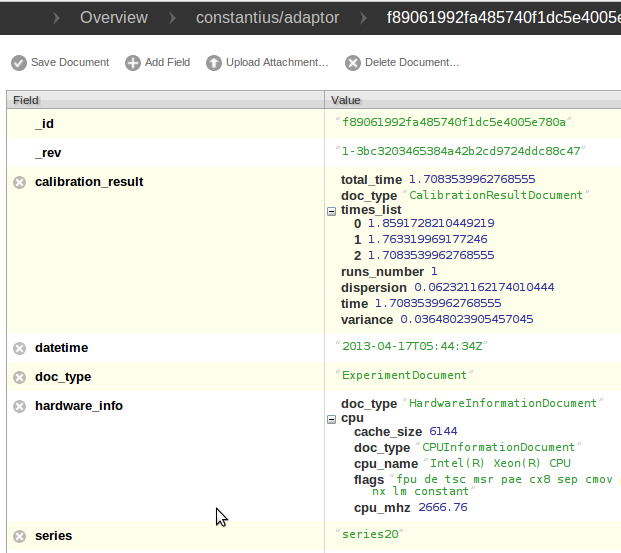
\includegraphics[width=\textwidth]{database-interaction}
			\end{figure}
		\end{column}
	\end{columns}
	
\end{frame}

\begin{frame}
\frametitle{Program building module}

	\begin{columns}[T]
		\begin{column}{0.5\textwidth}
			\begin{itemize}
				\item Manages paths to source files of experimental programs
				\begin{itemize}
					\item Sources are in hierarchical structure of directories
					\item Module enables that only specifying the name of program to build is enough for sources to be found
				\end{itemize}
				\item Manages build tools and their settings
			\end{itemize}
		\end{column}
		\begin{column}{0.5\textwidth}
			\begin{figure}
				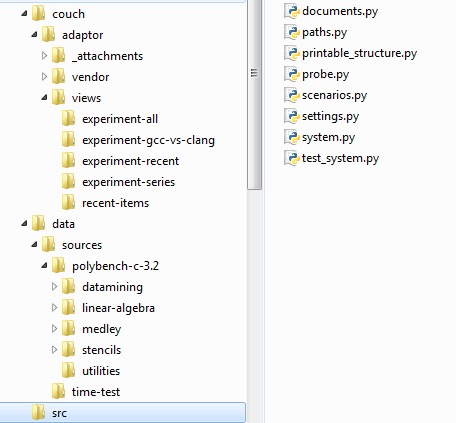
\includegraphics[width=\textwidth]{source-tree}
			\end{figure}
		\end{column}
	\end{columns}
	
\end{frame}

\begin{frame}
\frametitle{Experimentation module}

	\begin{columns}[T]
		\begin{column}{0.5\textwidth}
			\begin{itemize}
				\item Calibrates the program execution time measurement before every series of runs
				\begin{itemize}
					\item Subtracts the execution time of ''simplest'' program to avoid systematical error
					\item Runs the program being studied until relative  dispersion of time measurement becomes pretty low ($d_{rel} < 5\%$)
				\end{itemize}
				\item Passes the experiment data to the database interaction module
			\end{itemize}
		\end{column}
		\begin{column}{0.5\textwidth}
			\begin{figure}
				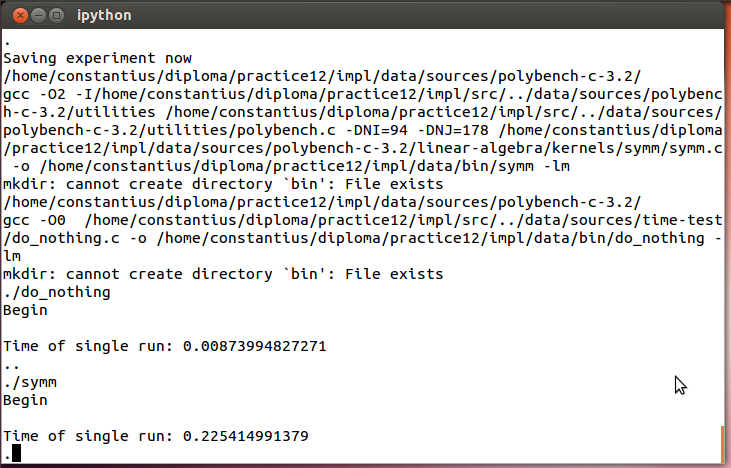
\includegraphics[width=\textwidth]{console}
			\end{figure}
		\end{column}
	\end{columns}
	
\end{frame}

\begin{frame}
\frametitle{Information retrieval module}

	\begin{columns}[T]
		\begin{column}{0.5\textwidth}
			\begin{itemize}
				\item Collects the information on used platform and experiment being carried out
				\item CPU
				\begin{itemize}
					\item Frequency
					\item Cache size
					\item Instruction set extensions
					\item etc.
				\end{itemize}

			\end{itemize}
		\end{column}
		\begin{column}{0.5\textwidth}
			\begin{itemize}
				\item Compiler
				\item Experiment
				\begin{itemize}
					\item Studied program
					\item Size of input data
				\end{itemize}
			\end{itemize}
		\end{column}
	\end{columns}
	
\end{frame}

\begin{frame}
\frametitle{Data analysis module}

\begin{itemize}
	\item Receives data from database and saves it to CSV files for input to \textit{Orange} statistical analysis system
	\item Graphs results using \textit{Python} library \textit{matplotlib}
	\item Two groups of program performance models
	\begin{itemize}
		\item Simplest (1 feature)
		\item More complex (3-5 features)
	\end{itemize}
	\item Four regression models in both groups
	\begin{itemize}
		\item Linear
		\item k Nearest Neighbors
		\item Multivariate Adaptive Regression Splines
		\item Random Forest
	\end{itemize}
\end{itemize}

\end{frame}

\begin{frame}
\frametitle{Data analysis module (cont.)}
	\begin{columns}[T]
	\begin{column}{0.5\textwidth}
		\begin{itemize}
			\item Scheme of 40 data analysis components in \textit{Orange} system
			\begin{itemize}
				\item Reading in
				\item Preprocessing
				\item Filtering
				\item Feature extraction
				\item Feature ranking
				\item Predictor fitting
				\item Prediction results evaluation
				\item Saving predictions to \textit{CSV} file
			\end{itemize}
		\end{itemize}
	\end{column}
	\begin{column}{0.5\textwidth}
		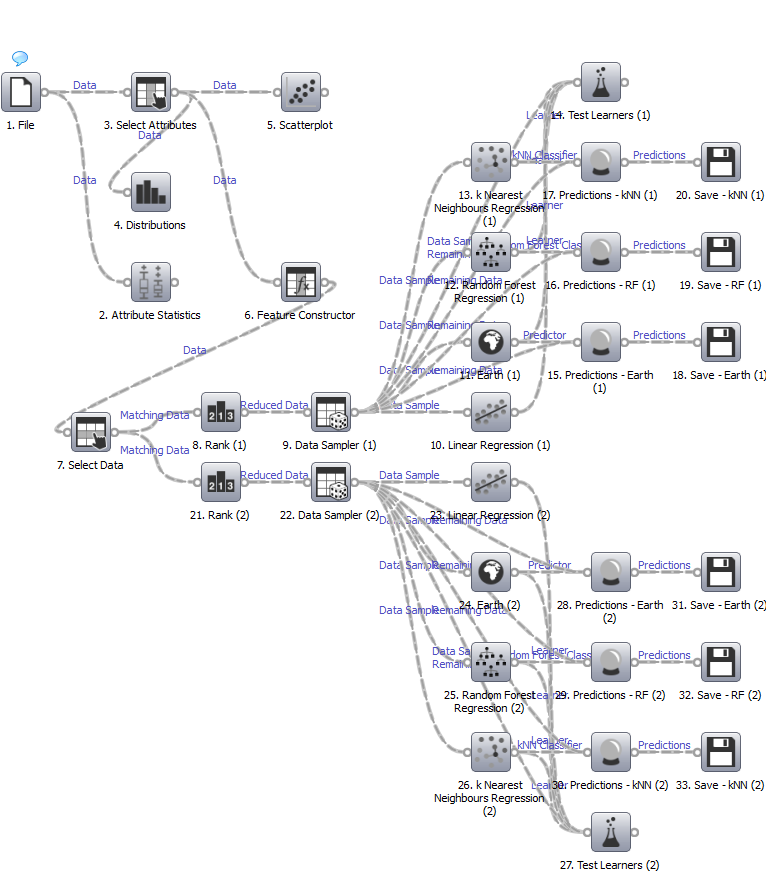
\includegraphics[width=\textwidth]{series30}
	\end{column}
	\end{columns}

\end{frame}

\section{Evaluation of implementation}
	\begin{columns}
		\begin{column}{0.5\textwidth}
			\begin{itemize}
				\item Platform
				\begin{itemize}
					\item \textit{Intel} CPUs
					\begin{itemize}
						\item \textit{Core 2 Quad Q8200} 2.33 GHz, 2 MB cache
						\item \textit{Core i5 M460} 2.53 GHz, 3 MB cache
						\item \textit{Xeon E5430} 2.66 GHz, 6 MB cache
					\end{itemize}
					\item \textit{Ubuntu 12.04}, \textit{gcc} and \textit{llvm} compilers
				\end{itemize}

				\item \textit{Polybench/C 3.2} benchmark set, 28 programs in total
				\begin{itemize}
					\item Linear algebra, solution of systems of linear algebraic equations and ordinary differential equations
				\end{itemize}
			\end{itemize}
		\end{column}
		\begin{column}{0.5\textwidth}
			\begin{itemize}
				\item Input data is generated by deterministic algorithms	
				\item Performance of chosen programs from benchmark set is modeled using \textit{Adaptor} framework
				\begin{itemize}
					\item \textit{symm}. Multiplication of symmetric matrices
					\begin{itemize}
						\item Square matrices of $2^i$ dimensionality, $i = f^{''}_{rand}(1,10)$
					\end{itemize}
				
					\item \textit{ludcmp}. LU-decomposition.
					\begin{itemize}
						\item Square matrices of $f^{''}_{rand}(2,1024)$ dimensionality
					\end{itemize}
				\end{itemize}
				
				\item 1000 experiments per CPU
			\end{itemize}
		\end{column}
	\end{columns}

\begin{frame}
\frametitle{Feature ranking. \textit{symm} program}

	\begin{columns}
		\begin{column}{0.5\textwidth}
			\begin{itemize}
				\item \textit{Earth Importance} selected only relevant features
			\end{itemize}
		\end{column}
		\begin{column}{0.5\textwidth}
			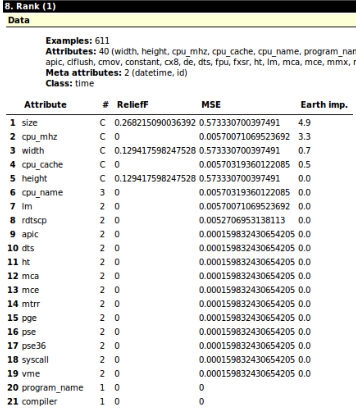
\includegraphics[scale=0.375]{feature-ranking}
		\end{column}	
	\end{columns}
	
\end{frame}

\begin{frame}
\frametitle{Feature ranking. \textit{symm} program (cont.)}

	\begin{columns}
		\begin{column}{0.5\textwidth}
			\begin{itemize}
				\item Root Relative Square Error of k Nearest Neighbors --- approx. 5\%
			\end{itemize}
		\end{column}
		\begin{column}{0.5\textwidth}
			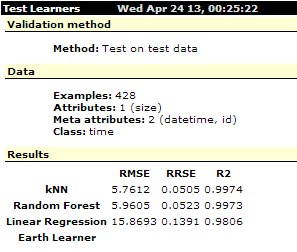
\includegraphics[scale=0.5]{evaluation-error}
		\end{column}	
	\end{columns}
	
\end{frame}

\begin{frame}
\frametitle{k Nearest Neighbors model of performance of \textit{symm} program on \textit{Q8200} CPU}
\begin{center}
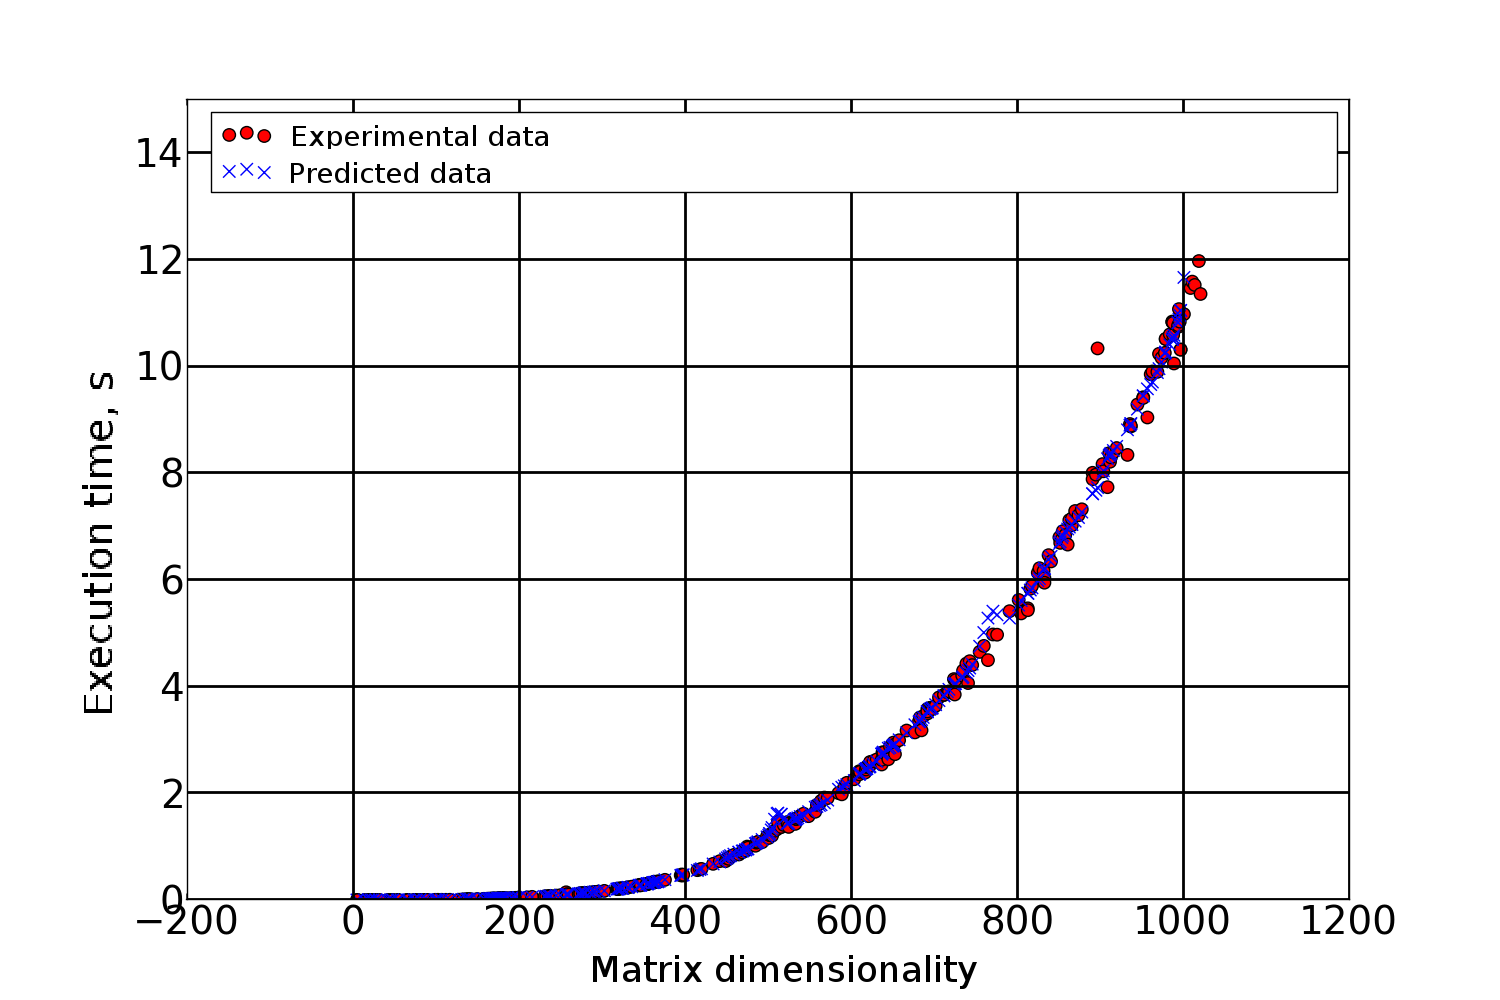
\includegraphics[scale=0.2]{symm-knn-q8200}
\end{center}
\end{frame}

\end{document}